\begin{center}

  \begin{tabular}{rp{16cm}lp{20cm}}%{rl}

  % after \\: \hline or \cline{col1-col2} \cline{col3-col4} ...

  论文地址:& \href{https://arxiv.org/pdf/2009.07111.pdf}{https://arxiv.org/pdf/2009.07111.pdf} \\
  来源:& AAAI, 2021\\
  作者:& Sheng Wan, Shirui Pan, Jian Yang, Chen Gong \\

  %源码:& \href{xxx}{xxx} \\

%  slides:& \href{http://yunshengb.com/wp-content/uploads/2017/03/nips_2018_r2l_workshop_talk.pdf}{{\footnotesize Convolutional Set Matching for Graph Similarity}}\\

  关键词:& \textbf{semi-supervised learning, GCN, Contrastive Learning} \\

  写于:& \date{2021-03-01}

  \end{tabular}

\end{center}

该论文\cite{wan2020contrastive}主要解决的是基于图的半监督学习中的监督信息短缺的问题,该论文结合数据之间的相似性和图结构来丰富监督信息。

\paragraph{问题定义}
假设共有$n=l+u$个样本(结点),$\Psi=\left\{\mathbf{x}_{1}, \cdots, \mathbf{x}_{l}, \mathbf{x}_{l+1}, \cdots, \mathbf{x}_{n}\right\}$,其中前$l$个样本为带标签的样本,标签为$\{y_i\}_{i=1}^l$,后$u$个样本不带标签,通常在半监督学习中$l$远小于$u$。特征矩阵为$\mathbf{X} \in \mathbb{R}^{n \times d}$,$\mathbf{Y} \in \mathbb{R}^{n \times c}$为标签矩阵。该论文的目标就是找到后$u$个结点的标签。(这是一个transductive的方法)。

\paragraph{思路}
\begin{figure}[h]
	\centering
	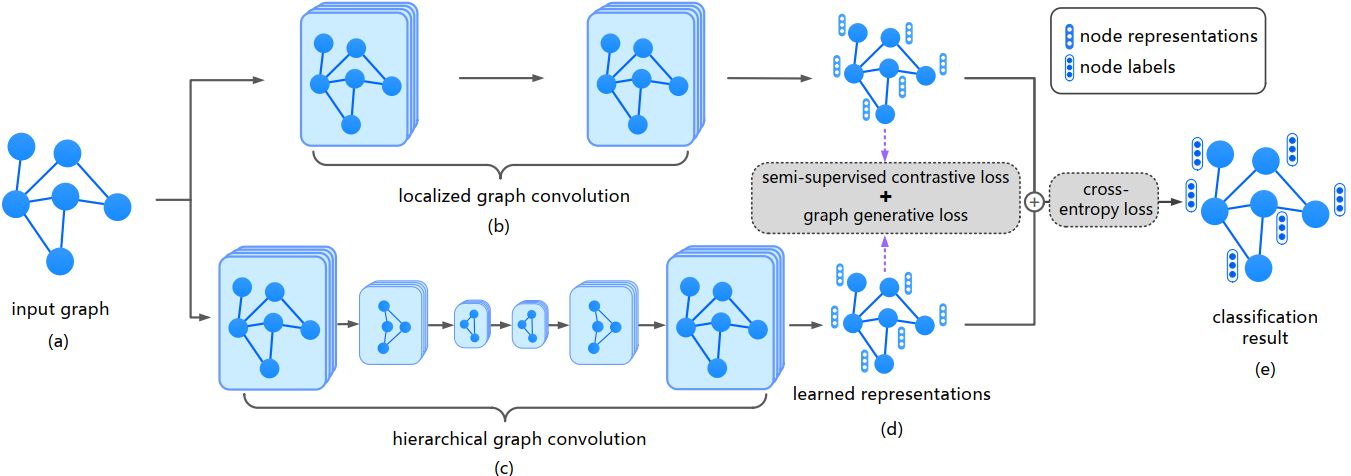
\includegraphics[width=.8\textwidth]{pics/CG3.png}
	\caption{CG3}
	\label{fig:cg3}
\end{figure}
整体框架如Fig.\ref{fig:cg3}所示。为了丰富监督信息,论文使用结点之间的相似性和图结构来丰富监督信息,分别使用半监督的对比学习来捕获数据之间的相似性和图生成损失来捕获图结构信息。

\subparagraph{Semi-Supervised Contrastive Learning}
对比学习通过数据之间的相似性与相异性来学习数据的表征,但是对比学习通常用在无标签数据中,不能利用标签数据。为此,论文中提出半监督的对比学习来利用带标签的数据。半监督的对比学习损失可以分为两部分:无监督的对比损失和监督的对比损失。

论文中使用local和global两种视角的GCN来生成结点表征(目的是为了后续的对比学习),分别表示为$\mathbf{H}^{\phi_1}, \mathbf{H}^{\phi_2}$。无监督的对比损失为:
$$
\mathcal{L}_{u c}=\frac{1}{2 n} \sum_{i=1}^{n}\left(\mathcal{L}_{u c}^{\phi_{1}}\left(\mathbf{x}_{i}\right)+\mathcal{L}_{u c}^{\phi_{2}}\left(\mathbf{x}_{i}\right)\right)
$$
其中$\mathcal{L}_{u c}^{\phi_{1}}\left(\mathbf{x}_{i}\right), \mathcal{L}_{u c}^{\phi_{2}}\left(\mathbf{x}_{i}\right)$分别为:
$$
\begin{array}{l}
\mathcal{L}_{u c}^{\phi_{1}}\left(\mathbf{x}_{i}\right)=-\log \frac{\exp \left(\left\langle\mathbf{h}_{i}^{\phi_{1}}, \mathbf{h}_{i}^{\phi_{2}}\right\rangle\right)}{\sum_{j=1}^{n} \exp \left(\left\langle\mathbf{h}_{i}^{\phi_{1}}, \mathbf{h}_{j}^{\phi_{2}}\right\rangle\right)}\\

\mathcal{L}_{u c}^{\phi_{2}}\left(\mathbf{x}_{i}\right)=-\log \frac{\exp \left(\left\langle\mathbf{h}_{i}^{\phi_{2}}, \mathbf{h}_{i}^{\phi_{1}}\right\rangle\right)}{\sum_{j=1}^{n} \exp \left(\left\langle\mathbf{h}_{i}^{\phi_{2}}, \mathbf{h}_{j}^{\phi_{1}}\right\rangle\right)}
\end{array}
$$

有监督的对比损失为:
$$
\mathcal{L}_{s c}=\frac{1}{2 l} \sum_{i=1}^{l}\left(\mathcal{L}_{s c}^{\phi_{1}}\left(\mathbf{x}_{i}\right)+\mathcal{L}_{s c}^{\phi_{2}}\left(\mathbf{x}_{i}\right)\right)
$$
其中$\mathcal{L}_{s c}^{\phi_{1}}\left(\mathbf{x}_{i}\right), \mathcal{L}_{s c}^{\phi_{2}}\left(\mathbf{x}_{i}\right)$分别为:
$$
\begin{array}{l}
	\mathcal{L}_{s c}^{\phi_{1}}\left(\mathbf{x}_{i}\right)=-\log \frac{\sum_{k=1}^{l} \mathbb{1}_{\left[y_{i}=y_{k}\right]} \exp \left(\left\langle\mathbf{h}_{i}^{\phi_{1}}, \mathbf{h}_{k}^{\phi_{2}}\right\rangle\right)}{\sum_{j=1}^{l} \exp \left(\left\langle\mathbf{h}_{i}^{\phi_{1}}, \mathbf{h}_{j}^{\phi_{2}}\right\rangle\right)} \\
	\mathcal{L}_{s c}^{\phi_{2}}\left(\mathbf{x}_{i}\right)=-\log \frac{\sum_{k=1}^{l} \mathbb{1}_{\left[y_{i}=y_{k}\right]} \exp \left(\left\langle\mathbf{h}_{i}^{\phi_{2}}, \mathbf{h}_{k}^{\phi_{1}}\right\rangle\right)}{\sum_{j=1}^{l} \exp \left(\left\langle\mathbf{h}_{i}^{\phi_{2}}, \mathbf{h}_{j}^{\phi_{1}}\right\rangle\right)},
\end{array}
$$

半监督对比损失为:$\mathcal{L}_{ssc} = \mathcal{L}_{uc} + \mathcal{L}_{sc}$。

\subparagraph{Graph Generative Loss}
为了利用图的结构作为监督信息引入了图生成损失。在现有生成模型的启示下,将图中边$e_{ij}$视为二元变量,并且该变量是条件独立的。所以在给定local和global视角的结点表征时,图的概率表示为:
$$
\begin{aligned}
	p(\mathcal{G} | \mathbf{H}^{\phi_1}, \mathbf{H}^{\phi_2}) = \prod_{i,j} p(e_{ij}| \mathbf{H}^{\phi_1}, \mathbf{H}^{\phi_2}) \\
	= \prod_{i,j} p(e_{ij}| \mathbf{h}_i^{\phi_1}, \mathbf{h}_j^{\phi_2}) \\
	= \prod_{i,j} \delta([\mathbf{h}_i^{\phi_1}, \mathbf{h}_j^{\phi_2}] \mathbb{w})
\end{aligned}
$$
(类似于极大似然概率),其中$\delta$为逻辑回归函数。

图生成损失为:$\mathcal{L}_{g^2} = - p(\mathcal{G} | \mathbf{H}^{\phi_1}, \mathbf{H}^{\phi_2})$。

\subparagraph{Model Training}
因为采用了local和global的视角,结点最终的表征为:$\mathbf{O} =f \lambda^{\phi_1}\mathbf{H}^{\phi_1} + (1-\lambda^{\phi_1})\mathbf{H}^{\phi_2}$。
因为还存在一部分带标签的数据,因此可以借助这一部分数据产生交叉熵损失:$\mathcal{L}_{ce} = -\sum_{i=1}^l \sum_{j=1}^c \mathbf{Y}_{ij} ln\mathbf{O}_{ij}$。
最终模型的损失即为:
$$
\mathcal{L} = \mathcal{L}_{ce} + \lambda_{ssc}\mathcal{L}_{ssc} + \lambda_{g^2}\mathcal{L}_{g^2}
$$
其中$\lambda_{ssc}, \lambda_{g^2}$均为超参数。

\paragraph{方法解决的问题/优势}

\begin{itemize}

	\item 将对比学习引入到半监督学习中,结合了不带标签的数据和带标签的数据
	\item 利用结点相似性与图结构来丰富监督信息

\end{itemize}



\paragraph{方法的局限性/未来方向}

\begin{itemize}

	\item 论文中的方法为transductive,不能应用于未见过的结点
	\item \tbc{red}{将论文中的方法改为inductive的}

\end{itemize}
